\documentclass{scu-thesis}
\usepackage{amsmath}	% for advanced typesetting of mathematics
\usepackage{graphicx}	% for including graphics
\usepackage{txfonts}	% for using the Times-Roman font
\usepackage{xcolor}
\usepackage{animate}

\usepackage[most]{tcolorbox} % for boxed content
\tcbset{
  colback=white,
  colframe=black,
  fonttitle=\bfseries,
  boxrule=0.5pt,
  arc=2mm,
  outer arc=1mm,
  coltitle=black,
  colbacktitle=gray!20,
  left=2mm,
  right=2mm,
  top=1mm,
  bottom=1mm,
}

\usepackage{graphicx}
\usepackage{caption}
\usepackage{float}

\usepackage[T1]{fontenc}
\usepackage[utf8]{inputenc} % utf8x is not supported by biblatex

% Bibliography
\usepackage[sorting=none, style=ieee, backend=biber]{biblatex}
\addbibresource{1150-references.bib}

% UML 
\usepackage{tikz}
\usepackage{tikz-uml}

\usepackage[most]{tcolorbox}
\usepackage{fullpage}
\usepackage{listings}

% Clickable table of contents, figure list and citations (load last)
\usepackage[hidelinks]{hyperref}

% These must be set first ... the rest of the thesis commands rely on them.

\author{David Chousal Cantu [CSEN]}
\author{Isabella Rodriguez [ECEN]}
\author{John Ryan Myrdal [GENG]}


% --- Project Title --- Project Title --- Project Title --- Project Title --- Project Title --- Project Title --- Project Title --- Project Title ---
\title{S.C.O.U.T.\texorpdfstring{\\}{ -- }Santa Clara Oceanic Utilities Transmitter}


\department{Department of Computer Science and Engineering}
\department{Department of Electrical and Computer Engineering}
\department{Department of General Engineering}
\degree{Bachelor of Science in Computer Science and Engineering}
\degree{Bachelor of Science in Electrical and Computer Engineering}
\degree{Bachelor of Science in General Engineering}

% Only bachelor's theses should have multiple authors and/or be from
% multiple departments.  Signatures required:
%
% Bachelor's theses: advisor(s), department chair(s)
% Master's theses: advisor, reader, department chair
% Doctoral theses: doctoral committee (including advisor), department chair

\begin{document}
\frontmatter
% Advisors (left) and department chairs (right) side by side so all six fit on one page
\noindent
\begin{minipage}[t]{0.49\textwidth}
\signature{Thesis Advisor Navid Shaghaghi [CSEN]}
\signature{Thesis Advisor Shoba Krishnan [ECEN]}
\signature{Thesis Advisor Jes Kuczenski [GENG]}
\end{minipage}\hfill
\begin{minipage}[t]{0.49\textwidth}
\signature{Department Chair Silvia Figueira [CSEN]}
\signature{Department Chair Shoba Krishnan [ECEN]}
\signature{Department Chair Matthew Gaudet [GENG]}
\end{minipage}

\maketitle
%     --- abstract --- abstract --- abstract --- abstract --- abstract --- abstract --- abstract --- abstract --- abstract --- 
\begin{abstract} % --- abstract --- abstract --- abstract --- abstract --- abstract --- abstract --- abstract --- abstract --- 
%     --- abstract --- abstract --- abstract --- abstract --- abstract --- abstract --- abstract --- abstract --- abstract --- 

\begin{tcolorbox}[      % Delete me later
    boxrule=0pt,        % Delete me later
    colback=white,      % Delete me later
    coltext=red         % Delete me later
]                       % Delete me later
    A good abstract is a concise summary (1--2 paragraphs) of the entire project: introduction, problem statement, work accomplished, results, conclusions, and recommendations. When you write the abstract, imagine that the reader will not read anything else but that you must get your major point across immediately. This requires the efficiency of words and phrases. An abstract is written to stand alone, without jargon or references to figures and tables in the report body.
    
    \vspace{15pt}           % Delete me later
    \begin{center}          % Delete me later
    \textbf{Don't forget to delete this explanatory red text/block introduction, and replace it with your text in black.}
    \end{center}            % Delete me later
\end{tcolorbox}
\end{abstract}


\tableofcontents % --- tableofcontents --- tableofcontents --- tableofcontents --- tableofcontents --- tableofcontents --- tableofcontents --- tableofcontents

\listoffigures % --- listoffigures --- listoffigures --- listoffigures --- listoffigures --- listoffigures --- listoffigures --- listoffigures --- listoffigures

\begin{tcolorbox}[      % Delete me later
    boxrule=0pt,        % Delete me later
    colback=white,      % Delete me later
    coltext=red         % Delete me later
]                       % Delete me later
    Overall, have at least 20 figures at the end of the senior design project. 
    
    \vspace{15pt}       % Delete me later
    \begin{center}      % Delete me later
    \textbf{Don't forget to delete this explanatory red text/block introduction, and replace it with your text in black.}
    \end{center}        % Delete me later
\end{tcolorbox}         % Delete me later

\mainmatter
%%%%%%%%%%%%%%%%%%%%%%%%%%%%%%%%%%%%%%%%%%%%%%%%%%%%%
%       --- Introduction --- Introduction --- Introduction --- Introduction --- Introduction --- Introduction --- Introduction --- Introduction ---
\chapter{Introduction} % --- Introduction --- Introduction --- Introduction --- Introduction --- Introduction --- Introduction --- Introduction --- 
%       --- Introduction --- Introduction --- Introduction --- Introduction --- Introduction --- Introduction --- Introduction --- Introduction --- 

Coral reefs are in steep decline. Since the 1950s, the global cover of living coral, and with it the capacity of reefs to provide food, coastal protection and income, has fallen by about half \cite{eddy2021}. Marine heatwaves now cause mass bleaching events that come back faster than reefs can recover \cite{hughes2017}, and sediment and nutrient runoff from land adds further stress to reefs close to shore \cite{fabricius2005}. Reef managers can only respond to stress they can see, which makes measuring the water around a reef the starting point of any protection effort.

Today most of that measuring is done from space. NOAA Coral Reef Watch uses satellite sea-surface temperature to warn of bleaching across the world's reefs \cite{liu2014}. Satellites cover the globe, but they are least reliable in shallow nearshore water, where land, the sea floor and coastal mixing distort the signal \cite{margaritis2025}. That nearshore water is exactly where many reefs live. In-water instruments close this gap, but they are expensive, and the data they record often reaches researchers only when someone travels out to collect the instrument.

This thesis presents S.C.O.U.T.\ (Santa Clara Oceanic Utilities Transmitter), a low-cost, battery-powered and modular monitoring buoy. It is moored next to a shallow reef and left alone for a year or more. It measures water temperature and turbidity, stores everything on board, and sends a short summary to a shore station every day over long-range, low-power radio. Coral reef health is its first application, and its first deployment is planned for a reef in Hawai'i in spring 2027. The rest of this chapter states the problem, the objectives that break it into steps, and the approach the team took.

%       --- Problem Statement --- Problem Statement --- Problem Statement --- Problem Statement --- Problem Statement ---
\section{Problem Statement} % --- Problem Statement --- Problem Statement --- Problem Statement --- Problem Statement ---
%       --- Problem Statement --- Problem Statement --- Problem Statement --- Problem Statement --- Problem Statement ---

In the summer of 2026 the team interviewed three NOAA coral reef researchers about how reefs are monitored today and where that monitoring falls short. Their answers pointed to the same gap. Nearshore reef water is poorly measured, because satellite products are least accurate there and in-water instruments are too costly to deploy widely. Advanced monitoring buoys can cost tens of thousands of dollars. Simpler loggers are cheaper, but they store their data internally, so researchers see it only when a diver recovers the logger. At remote sites that can mean a wait of several years, which rules out responding to a bleaching event or a sediment plume while it is happening. Every service visit also costs boat time and dive time, so an instrument that needs frequent care is unlikely to stay in the water.

The problem this project addresses can therefore be stated as follows. Coral reef researchers and managers need an affordable instrument that measures water conditions at a shallow reef and delivers those measurements to shore while the reef is still being watched, subject to the following criteria:
\begin{enumerate}
    \item \textbf{Cost.} The complete system must cost well below \$5{,}000 per buoy, the figure the interviewed researchers named as the practical limit for deploying instruments at many sites.
    \item \textbf{Endurance.} The buoy must run unattended for at least one year, with no recharging, battery change or cleaning visit in that time.
    \item \textbf{Data access.} Measurements must reach a shore station at least once a day, without relying on cellular coverage or an internet connection at the buoy.
    \item \textbf{Measurements.} The buoy must measure, at minimum, water temperature and turbidity at reef depths of 2 to 8\,m, the two signals the researchers valued most, and must accept further sensors, starting with an underwater microphone for reef sound.
    \item \textbf{Survival.} The buoy must stay afloat, moored and watertight in nearshore waves, salt water and biological growth for the full deployment.
    \item \textbf{Usable output.} The data must arrive in a form researchers can use directly, such as the heat-stress measure used by NOAA Coral Reef Watch, rather than as raw sensor readings.
\end{enumerate}
These criteria define the scope of the work. A buoy that meets all six gives researchers in-water measurements from the places satellites see least clearly, at a cost that allows many buoys instead of one.

%       --- Background or Related Work --- Background or Related Work --- Background or Related Work --- Background or Related Work ---
\section{Background or Related Work} % --- Background or Related Work --- Background or Related Work --- Background or Related Work ---
%       --- Background or Related Work --- Background or Related Work --- Background or Related Work --- Background or Related Work ---

\begin{tcolorbox}[      % Delete me later
    boxrule=0pt,        % Delete me later
    colback=white,      % Delete me later
    coltext=red         % Delete me later
]                       % Delete me later
    State who else has worked on this problem or similar problems (you should do most of your citations here). For applied projects, provide information on other existing programs which will use your program.
    
    Describe what systems already exist and why they are inadequate. 
    
    \vspace{15pt}       % Delete me later
    \begin{center}      % Delete me later
    \textbf{Don't forget to delete this explanatory red text/block introduction, and replace it with your text in black.}
    \end{center}        % Delete me later
\end{tcolorbox}         % Delete me later

%       --- Objectives --- Objectives --- Objectives --- Objectives --- Objectives --- Objectives --- Objectives --- Objectives --- Objectives
\section{Objectives} % --- Objectives --- Objectives --- Objectives --- Objectives --- Objectives --- Objectives --- Objectives --- Objectives
%       --- Objectives --- Objectives --- Objectives --- Objectives --- Objectives --- Objectives --- Objectives --- Objectives --- Objectives

The project goals are broken into the following objectives. Each one produces a result that can be checked, and together they lead from requirements to a buoy working at a real reef. They follow the phases of the project timeline, which runs from August 2026 to May 2027.
\begin{enumerate}
    \item \textbf{Set the requirements.} Turn the researcher interviews into measurable requirements for cost, endurance, sensing, data delivery and survival, and record each design decision as it is made.
    \item \textbf{Bring up each subsystem on the bench.} Get the microcontroller and radio, the temperature sensor, the turbidity sensor, the real-time clock and the memory card working one at a time, and measure how much current each one draws.
    \item \textbf{Write the buoy firmware.} Build software that sleeps between readings, wakes about every 30 minutes to measure, saves every reading to the memory card, sends three short radio packets a day, and restarts itself if it ever freezes.
    \item \textbf{Size the power system.} Use the measured currents to confirm that two non-rechargeable lithium D cells can run the buoy for at least one year, with margin.
    \item \textbf{Build the shore side.} Build a shore station that receives the buoy's packets and forwards them over WiFi, and a dashboard that shows the data along with bleaching heat stress and turbidity alerts.
    \item \textbf{Design the buoy body.} Design and 3D-print the floating hull, a sealed electronics housing and a sensor pod, and plan the mooring, then check that the housing stays dry under pressure equal to 5\,m of water.
    \item \textbf{Integrate and test.} Combine the subsystems into one buoy and test it in stages: on the bench, submerged in a tank, at a local dock and in a field prototype deployment in early 2027.
    \item \textbf{Deploy and evaluate.} Deploy the buoy at a reef in Hawai'i from March to May 2027 and compare its readings with established NOAA temperature records to judge how accurate they are.
\end{enumerate}
Objectives 2 to 6 are split among the three disciplines on the team: computer science and engineering for the firmware and shore software, electrical and computer engineering for the circuits and power, and general engineering for the hull, housing and mooring. Objectives 1, 7 and 8 are shared by the whole team.

%       --- Our approach --- Our approach --- Our approach --- Our approach --- Our approach --- Our approach --- Our approach --- Our approach --- 
\section{Our approach} % --- Our approach --- Our approach --- Our approach --- Our approach --- Our approach --- Our approach --- Our approach --- 
%       --- Our approach --- Our approach --- Our approach --- Our approach --- Our approach --- Our approach --- Our approach --- Our approach --- 

The team's approach rests on one idea: if the buoy uses very little energy and needs no care, it can be built from inexpensive parts and still stay in the water for a year. Every design choice is judged first by how it affects power use and maintenance, and only then by features.

\textbf{Low-cost, widely available parts.} The buoy is built around an Adafruit Feather M0 board with an RFM95 LoRa radio, a DS18B20 digital temperature sensor and an optical turbidity sensor. These are inexpensive parts with public documentation, so a damaged buoy can be repaired or copied without a specialist supplier. The hull and housings are 3D-printed, which keeps tooling costs at zero and lets the team change the design between tests.

\textbf{Sleep most of the time.} The buoy spends nearly all of its life asleep. About every 30 minutes it wakes, takes its readings, saves them and goes back to sleep. The turbidity sensor is switched off completely between readings. This is what allows two non-rechargeable lithium D cells to replace the solar panel and rechargeable battery of earlier designs. Removing the panel also removes the part most exposed to waves and biological growth.

\textbf{Send summaries, not raw data.} The buoy keeps its full record on a memory card and sends only a 44-byte summary over the radio, three times a day. LoRa radio was chosen because it reaches several kilometers on very little power and has been shown to work over seawater \cite{jovalekic2018}, including from antennas mounted at buoy height \cite{parri2019}. Small, infrequent packets keep the radio's share of the energy budget very low and need no cellular network or license fees.

\textbf{Turn readings into reef information.} On shore, the software applies the same heat-stress calculation that NOAA Coral Reef Watch uses with satellite data \cite{liu2014}, but feeds it temperatures measured in the water at the reef. Researchers therefore see bleaching risk for their own site, measured where satellites are least accurate, alongside turbidity trends and alerts.

\textbf{A platform, not a single instrument.} The sensors sit in a separate pod below the main electronics housing, so new sensors can be added without redesigning the hull or the electronics. An underwater microphone is the first planned addition, and the radio packet already carries a short summary of reef sound.

Together these choices set S.C.O.U.T.\ apart from existing options. It costs far less than an advanced monitoring buoy, it reports every day instead of waiting for a diver to recover a logger, and it measures the nearshore water that satellite products describe least reliably. The goal is not to replace existing monitoring networks but to make in-water measurements cheap enough to place at many more reefs.

%              --- User Research --- User Research --- User Research --- User Research --- User Research --- User Research --- User Research ---
\chapter{User Research - example middle chapter} % --- User Research --- User Research --- User Research --- User Research --- User Research ---
%              --- User Research --- User Research --- User Research --- User Research --- User Research --- User Research --- User Research ---

%       --- Methods --- Methods --- Methods --- Methods --- Methods --- Methods --- Methods --- Methods --- Methods --- Methods --- Methods --- Methods 
\section{Methods} % --- Methods --- Methods --- Methods --- Methods --- Methods --- Methods --- Methods --- Methods --- Methods --- Methods --- Methods 
%       --- Methods --- Methods --- Methods --- Methods --- Methods --- Methods --- Methods --- Methods --- Methods --- Methods --- Methods --- Methods 

\begin{tcolorbox}[      % Delete me later
    boxrule=0pt,        % Delete me later
    colback=white,      % Delete me later
    coltext=red         % Delete me later
]                       % Delete me later
    Describe what methods you have used to identify user needs. This can include methods such as storyboards and interviews and surveys with target users. Describe how you analyze the data you collect. Include an example. 
    
    \vspace{15pt}       % Delete me later
    \begin{center}      % Delete me later
    \textbf{Don't forget to delete this explanatory red text/block introduction, and replace it with your text in black.}
    \end{center}        % Delete me later
\end{tcolorbox}         % Delete me later

%       --- Stakeholder needs --- Stakeholder needs --- Stakeholder needs --- Stakeholder needs --- Stakeholder needs --- Stakeholder needs ---
\section{Stakeholder needs} % --- Stakeholder needs --- Stakeholder needs --- Stakeholder needs --- Stakeholder needs --- Stakeholder needs ---
%       --- Stakeholder needs --- Stakeholder needs --- Stakeholder needs --- Stakeholder needs --- Stakeholder needs --- Stakeholder needs ---

\begin{tcolorbox}[      % Delete me later
    boxrule=0pt,        % Delete me later
    colback=white,      % Delete me later
    coltext=red         % Delete me later
]                       % Delete me later
    Who are the stakeholders for this system? Provide a short description of what you know (so far) about each of the stakeholders and their needs. Highlight cases where their needs may differ. Personas could be appropriate here.
    
    Describe whose needs your system will prioritize. It is ok to state that a potential stakeholder is out of scope for the project. For example, a virtual tour of the SCU campus might target prospective students, but choose \textit{not} optimize for their parents (who are also potential stakeholders/viewers, but have different needs).

    \vspace{15pt}       % Delete me later
    \begin{center}      % Delete me later
    \textbf{Don't forget to delete this explanatory red text/block introduction, and replace it with your text in black.}
    \end{center}        % Delete me later
\end{tcolorbox}         % Delete me later

%       --- User stories --- User stories --- User stories --- User stories --- User stories --- User stories --- User stories --- User stories ---
\section{User stories} % --- User stories --- User stories --- User stories --- User stories --- User stories --- User stories --- User stories ---
%       --- User stories --- User stories --- User stories --- User stories --- User stories --- User stories --- User stories --- User stories ---

\begin{tcolorbox}[      % Delete me later
    boxrule=0pt,        % Delete me later
    colback=white,      % Delete me later
    coltext=red         % Delete me later
]                       % Delete me later
    For each stakeholder that you choose to prioritize, describe one or more user stories that your system will support, e.g., "As a prospective student, I want to find a social group at SCU so that I have friends to hang out with."
    
    Based on our user research and the priority stakeholders, we formulate the following user stories to guide system design. Each story captures a specific goal from a stakeholder's perspective and informs both feature planning and testing.
    
    \subsubsection*{Prospective Students}
    \begin{itemize}
      \item \textbf{As a prospective student,} I want to take a virtual tour of SCU’s dorms, \textbf{so that} I can compare housing options before visiting campus.
      \item \textbf{As a prospective student,} I want to preview clubs and student groups, \textbf{so that} I can plan how to get involved socially.
    \end{itemize}
    
    \subsubsection*{Parents of Prospective Students}
    \begin{itemize}
      \item \textbf{As a parent,} I want to access safety and health information during the tour, \textbf{so that} I feel confident in my child’s well-being on campus.
      \item \textbf{As a parent,} I want to know about academic support services, \textbf{so that} I can trust the school’s ability to help my child succeed.
    \end{itemize}
    
    \subsubsection*{Admissions Officers}
    \begin{itemize}
      \item \textbf{As an admissions officer,} I want to update featured content on the tour, \textbf{so that} we can highlight new programs each quarter.
      \item \textbf{As an admissions officer,} I want to track which parts of the tour are most visited, \textbf{so that} I can refine our outreach strategy.
    \end{itemize}
    
    \subsubsection*{Student Tour Guides}
    \begin{itemize}
      \item \textbf{As a student ambassador,} I want to record guided walkthroughs of campus spots, \textbf{so that} I can offer a personal touch remotely.
    \end{itemize}
    \vspace{15pt}       % Delete me later
    \begin{center}      % Delete me later
    \textbf{Don't forget to delete this explanatory red text/block introduction, and replace it with your text in black.}
    \end{center}        % Delete me later
\end{tcolorbox}         % Delete me later
%       --- Design and Rationale --- Design and Rationale --- Design and Rationale --- Design and Rationale --- Design and Rationale --- Design and Rationale
\chapter{Design and Rationale - example middle chapter} % --- Design and Rationale --- Design and Rationale --- Design and Rationale --- Design and Rationale
%       --- Design and Rationale --- Design and Rationale --- Design and Rationale --- Design and Rationale --- Design and Rationale --- Design and Rationale

%       --- Design --- Design --- Design --- Design --- Design --- Design --- Design --- Design --- Design --- Design --- Design --- Design --- Design ---
\section{Design} % --- Design --- Design --- Design --- Design --- Design --- Design --- Design --- Design --- Design --- Design --- Design --- Design ---
%       --- Design --- Design --- Design --- Design --- Design --- Design --- Design --- Design --- Design --- Design --- Design --- Design --- Design ---

\begin{tcolorbox}[      % Delete me later
    boxrule=0pt,        % Delete me later
    colback=white,      % Delete me later
    coltext=red         % Delete me later
]                       % Delete me later
    Describe the design of the system at a high level. The system should support the use cases described in the previous chapter.
    
    ---C4 system context and container diagrams go in this section. See: https://c4model.com/ (C4 Model Website)

    \vspace{15pt}       % Delete me later
    \begin{center}      % Delete me later
    \textbf{Don't forget to delete this explanatory red text/block introduction, and replace it with your text in black.}
    \end{center}        % Delete me later
\end{tcolorbox}         % Delete me later

\pagebreak

%       --- Use Case Overview --- Use Case Overview --- Use Case Overview --- Use Case Overview --- Use Case Overview --- Use Case Overview ---
\section{Use Case Overview} % --- Use Case Overview --- Use Case Overview --- Use Case Overview --- Use Case Overview --- Use Case Overview ---
%       --- Use Case Overview --- Use Case Overview --- Use Case Overview --- Use Case Overview --- Use Case Overview --- Use Case Overview ---

\begin{tcolorbox}[      % Delete me later
    boxrule=0pt,        % Delete me later
    colback=white,      % Delete me later
    coltext=red         % Delete me later
]                       % Delete me later
    Brief explanation of how use cases were derived from user stories.

    \vspace{15pt}       % Delete me later
    \begin{center}      % Delete me later
    \textbf{Don't forget to delete this explanatory red text/block introduction, and replace it with your text in black.}
    \end{center}        % Delete me later
\end{tcolorbox}         % Delete me later

%       --- Use Case Descriptions --- Use Case Descriptions --- Use Case Descriptions --- Use Case Descriptions ---
\section{Use Case Descriptions} % --- Use Case Descriptions --- Use Case Descriptions --- Use Case Descriptions ---
%       --- Use Case Descriptions --- Use Case Descriptions --- Use Case Descriptions --- Use Case Descriptions ---

\begin{figure}[h!]
    \centering
    \begin{tcolorbox}[title=Use Case 1: EXAMPLE Explore Campus Virtually]
        \textbf{Actor:} Prospective Student
        \textbf{Preconditions:} User is on the landing page.

        \textbf{Main Flow:}
        \begin{enumerate}
            \item User selects “Start Virtual Tour”.
            \item System displays a map of campus buildings.
            \item User clicks on a building icon.
            \item System opens a 3D or 360° tour of that building.
        \end{enumerate}

        \textbf{Alternate Flow:} If media fails to load, fallback images are shown.
        \textbf{Postconditions:} User has explored one or more buildings virtually.
    \end{tcolorbox}

    \vspace*{-5pt}
    \caption{Use Case 1: EXAMPLE Explore Campus Virtually}
    \label{fig:usecase1}
\end{figure}

\vspace{1em}

\begin{figure}[h!]
    \centering
    \begin{tcolorbox}[title=Use Case 2: EXAMPLE View Campus Safety Information]
        \textbf{Actor:} Parent of Prospective Student
        \textbf{Preconditions:} User is on the main information page.

        \textbf{Main Flow:}
        \begin{enumerate}
            \item User navigates to the “Safety Info” section.
            \item System displays emergency contacts and safety resources.
        \end{enumerate}

        \textbf{Postconditions:} User is informed about campus safety services.
    \end{tcolorbox}

    \vspace*{-5pt}
    \caption{Use Case 2:  EXAMPLE View Campus Safety Information}
    \label{fig:usecase2}
\end{figure}

\pagebreak

%         --- Use Case Diagram --- Use Case Diagram --- Use Case Diagram --- Use Case Diagram --- Use Case Diagram ---
%         --- Use Case Diagram --- Use Case Diagram --- Use Case Diagram --- Use Case Diagram --- Use Case Diagram ---
\section{Use Case Diagram(s)} % --- Use Case Diagram --- Use Case Diagram --- Use Case Diagram --- Use Case Diagram ---

\begin{tcolorbox}[      % Delete me later
    boxrule=0pt,        % Delete me later
    colback=white,      % Delete me later
    coltext=red         % Delete me later
]                       % Delete me later
    Include at least one UML use case diagram that includes an overview and relationship of your text use cases.
    \vspace{\baselineskip}
    (You can use the tikz-uml package to draw a Unified Modeling Language models or you use an UML editor of your choice and upload the pictures here.)
    
    \vspace{15pt}       % Delete me later
    \begin{center}      % Delete me later
    \textbf{Don't forget to delete this explanatory red text/block introduction, and replace it with your text in black.}
    \end{center}        % Delete me later
\end{tcolorbox}         % Delete me later



\begin{figure}[h!] % Use Case Diagram ---
    \centering
    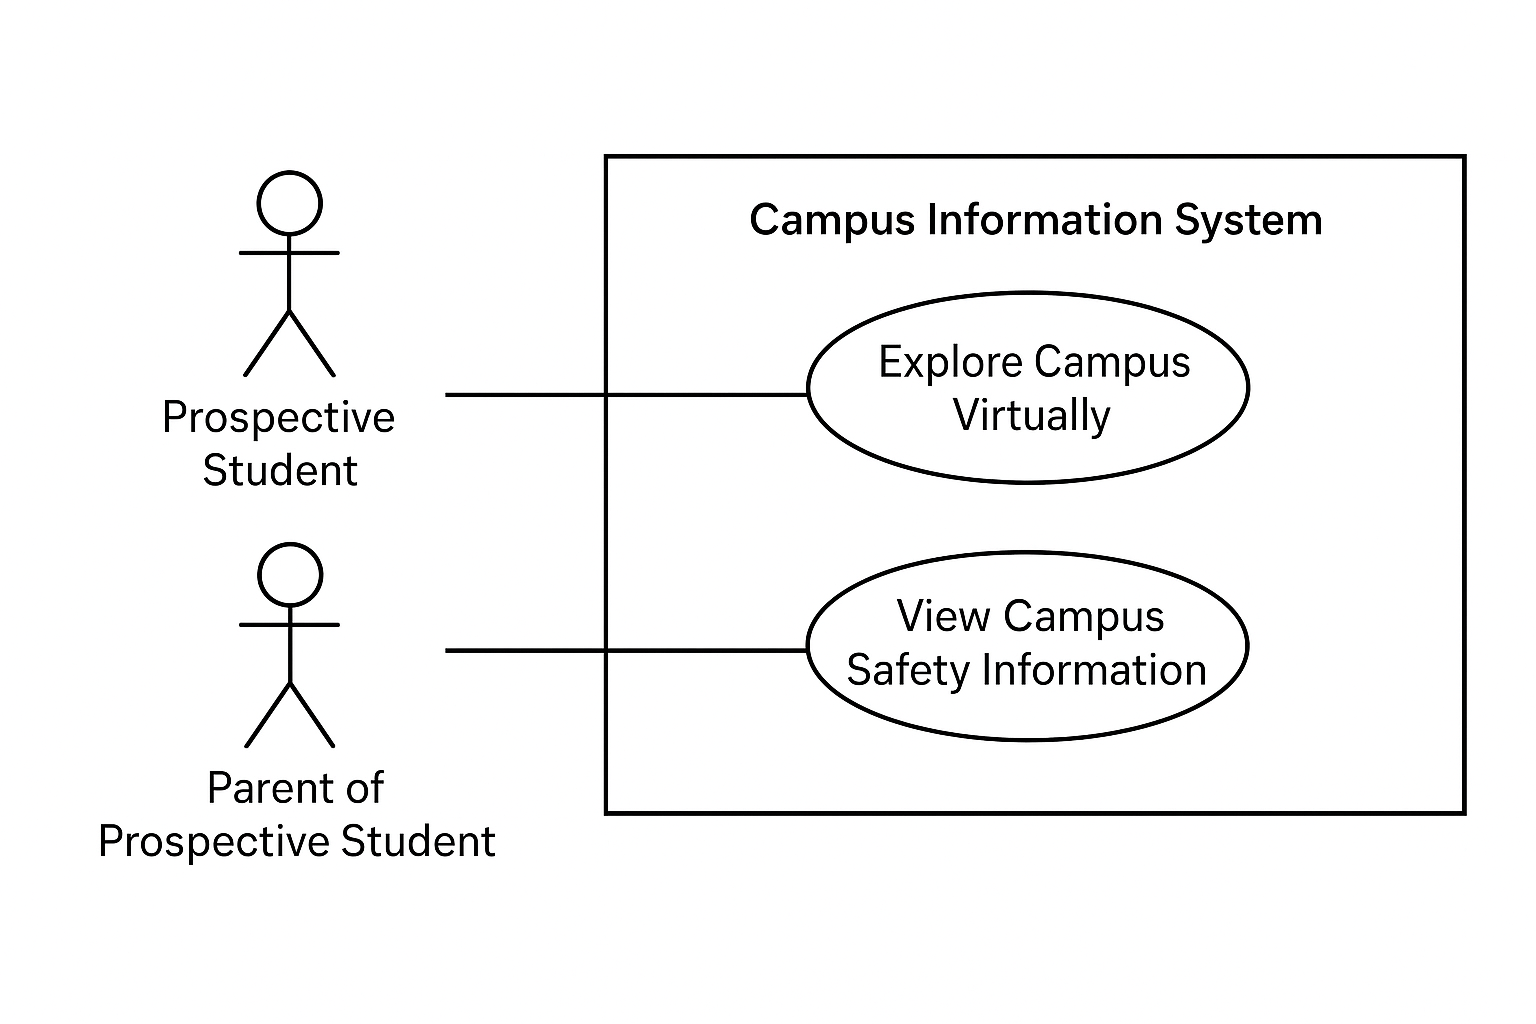
\includegraphics[width=0.8\linewidth]{pictures/example-use-case-diagram.png}

% For some reasons drawing UML Use Case diagrams with tik looks ugly, so picture included (above)
%    \begin{tikzpicture}
%        \begin{umlpackage}{Campus Information System}
%            % Use cases inside
%            \umlusecase[x=4,y=3.5,width=4cm]{Explore Campus Virtually}
%            \umlusecase[x=4,y=1,width=4cm]{View Campus Safety Information}
%        \end{umlpackage}
%        
%        % Actors outside (aligned left)
%        \umlactor[x=0,y=3.5]{Prospective Student}
%        \umlactor[x=0,y=1]{Parent of Prospective Student}
%        
%        % Associations (straight connections)
%        \umlassoc{Prospective Student}{usecase-1}
%        \umlassoc{Parent of Prospective Student}{usecase-2}
%    \end{tikzpicture}

    \caption{EXAMPLE UML Use Case Diagram: Campus Information System}
    \label{fig:uml_use_case_diagram}
\end{figure}


    
\pagebreak

%       --- Class Diagram --- Class Diagram --- Class Diagram --- Class Diagram --- Class Diagram ---
\section{Class Diagram} % --- Class Diagram --- Class Diagram --- Class Diagram --- Class Diagram ---
%       --- Class Diagram --- Class Diagram --- Class Diagram --- Class Diagram --- Class Diagram ---

\begin{tcolorbox}[      % Delete me later
    boxrule=0pt,        % Delete me later
    colback=white,      % Delete me later
    coltext=red         % Delete me later
]                       % Delete me later
    Include at least one UML Class Diagram that includes an overview over your system.
    
    \vspace{\baselineskip}
    (You can use the tikz-uml package to draw a Unified Modeling Language models or you use an UML editor of your choice and upload the pictures here.)

    \vspace{15pt}       % Delete me later
    \begin{center}      % Delete me later
    \textbf{Don't forget to delete this explanatory red text/block introduction, and replace it with your text in black.}
    \end{center}        % Delete me later
\end{tcolorbox}         % Delete me later


\begin{figure}[h!] % Class Diagram ---
    \centering
    \begin{center}
        \begin{tikzpicture}
            \begin{umlpackage}{System}
                \begin{umlpackage}{UserRegistration}
                    \umlclass[template=T]{User}{
                        age : uint
                        \\
                        birthday : Date
                    }{}
                    \umlclass[y=-3]{Department}{
                        d : double
                    }{
                        \umlvirt{
                            setB(b : B) : void
                        } 
                        \\ 
                        getB() : B
                    }
                \end{umlpackage}
            
                \begin{umlpackage}[x=10,y=-6]{Facility}
                    \umlinterface{BaseBuilding}{
                        n : uint 
                        \\ 
                        s : string
                    }{}
                \end{umlpackage}
            
                \umlclass[x=2,y=-10]{DataType}{
                    n : uint
                }{}
            \end{umlpackage}
            
            \umlassoc[geometry=-|-, arg1=tata, mult1=*, pos1=0.3, arg2=toto, mult2=1, pos2=2.9, align2=left]{BaseBuilding}{Department}
            \umlunicompo[geometry=-|, arg=titi, mult=*, pos=1.7, stereo=vector]{DataType}{BaseBuilding}
            \umlimport[geometry=|-, anchors=90 and 50, name=import]{Facility}{UserRegistration}
            \umlaggreg[arg=tutu, mult=1, pos=0.8, angle1=30, angle2=60, loopsize=2cm]{DataType}{DataType}
            \umlinherit[geometry=-|]{DataType}{Department}
            \umlnote[x=2.5,y=-6, width=3cm]{Department}{Every department has at least one user}
            \umlnote[x=7.5,y=-2]{import-2}{This note is about the import relationship.}
        \end{tikzpicture}
    \end{center}
    \caption{EXAMPLE Class Diagram: System}
    \label{fig:class_diagram}
\end{figure}

\pagebreak

%       --- Sequence Diagram --- Sequence Diagram --- Sequence Diagram --- Sequence Diagram --- Sequence Diagram ---
\section{Sequence Diagram} % --- Sequence Diagram --- Sequence Diagram --- Sequence Diagram --- Sequence Diagram ---
%       --- Sequence Diagram --- Sequence Diagram --- Sequence Diagram --- Sequence Diagram --- Sequence Diagram ---

\begin{figure}[h!] % Sequence Diagram ---
    \centering
    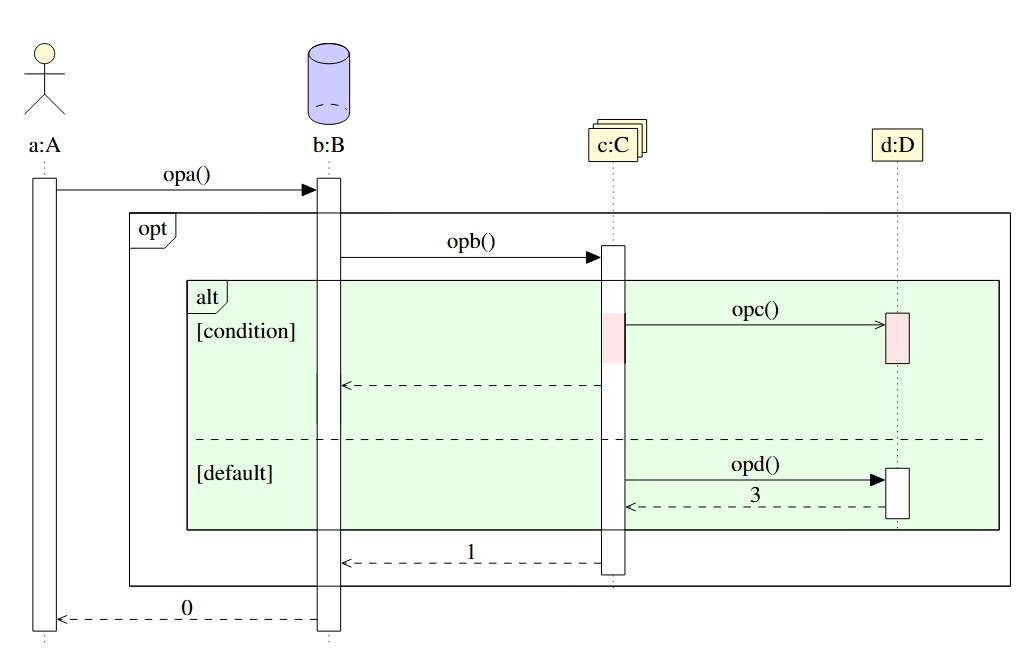
\includegraphics[width=0.8\linewidth]{pictures/example-sequence-diagram.jpg}
    
%    For some reason, this TIK creates two if-then-else errors 
%    \begin{tikzpicture}
%        \begin{umlseqdiag}
%            \umlactor[class=A]{a}
%            \umldatabase[class=B, fill=blue!20]{b}
%            \umlmulti[class=C]{c}
%            \umlobject[class=D]{d}
%            \begin{umlcall}[op=opa(), type=synchron, return=0]{a}{b}
%                \begin{umlfragment}
%                    \begin{umlcall}[op=opb(), type=synchron, return=1]{b}{c}
%                        \begin{umlfragment}[type=alt, label=condition, inner xsep=8, fill=green!10]
%                            \begin{umlcall}[op=opc(), type=asynchron, fill=red!10]{c}{d}
%                            \end{umlcall}
%                            \begin{umlcall}[type=return]{c}{b}
%                            \end{umlcall}
%                            \umlfpart[default]
%                            \begin{umlcall}[op=opd(), type=synchron, return=3]{c}{d}
%                            \end{umlcall}
%                        \end{umlfragment}
%                    \end{umlcall}
%                \end{umlfragment}
%            \end{umlcall}
%        \end{umlseqdiag}
%    \end{tikzpicture}
    \caption{EXAMPLE Sequence Diagram: Security Hand Shake}
    \label{fig:sequence_diagram}
\end{figure}

\pagebreak

%       --- State Diagram --- State Diagram --- State Diagram --- State Diagram --- State Diagram --- State Diagram ---
\section{State Diagram} % --- State Diagram --- State Diagram --- State Diagram --- State Diagram --- State Diagram ---
%       --- State Diagram --- State Diagram --- State Diagram --- State Diagram --- State Diagram --- State Diagram ---

\begin{figure}[h!] % State Diagram ---
    \centering
    \begin{center}
        \begin{tikzpicture}
            \begin{umlstate}[name=Amain]{Initialization Process}
                \begin{umlstate}[name=Bgraph, fill=red!20]{graphe B}
                    \umlstateinitial[name=Binit]
                    \umlbasicstate[y=-4, name=test1, fill=white]{test1}
                    \umltrans{Binit}{test1}
                    \umltrans[recursive=20|60|2.5cm, recursive direction=right to top, arg={op1}, pos=1.5]{test1}{test1}
                    \umltrans[recursive=160|120|2.5cm, recursive direction=left to top, arg={op2}, pos=1.5]{test1}{test1}
                    \umltrans[recursive=-160|-120|2.5cm, recursive direction=left to bottom, arg={op3}, pos=1.5]{test1}{test1}
                    \umltrans[recursive=-20|-60|2.5cm, recursive direction=right to bottom, arg={op4}, pos=1.5]{test1}{test1}
                    \umlbasicstate[y=-8, name=test2, fill=white]{test2}
                    \umltrans[recursive=-160|-120|2.5cm, recursive direction=left to bottom, arg={op5}, pos=1.5]{test2}{test2}
                    \umltrans{test1}{test2}
                    \umlstatefinal[x=3, y=-7.75, name=Bfinal]
                    \umltrans{test2}{Bfinal}
            \end{umlstate}
                \umlstateinitial[x=6, y=1, name=Ainit]
                \umlVHtrans[anchor2=40]{Ainit}{Bgraph}
                \umlstatefinal[x=6, y=-3.5, name=Afinal]
                \umlHVtrans[anchor1=30]{Bgraph}{Afinal}
                \umlbasicstate[x=6, y=-6, name=visu, fill=green!20]{Visualisation}
                \umlHVtrans{Bfinal}{visu}
                \umltrans{visu}{Afinal}
                \umltrans[recursive=-20|-60|2.5cm, recursive direction=right to bottom, arg=a, pos=1.5]{visu}{visu}
            \end{umlstate}
        \end{tikzpicture}
    \end{center}
    \caption{EXAMPLE State Diagram: Initialization Process}
    \label{fig:state_diagram}
\end{figure}

\pagebreak

%       --- Component Diagram --- Component Diagram --- Component Diagram --- Component Diagram --- Component Diagram --- Component Diagram ---
\section{Component Diagram} % --- Component Diagram --- Component Diagram --- Component Diagram --- Component Diagram --- Component Diagram ---
%       --- Component Diagram --- Component Diagram --- Component Diagram --- Component Diagram --- Component Diagram --- Component Diagram ---

\begin{figure}[h!] % Component Diagram ---
    \centering
    \begin{center}
        \begin{tikzpicture}
            \begin{umlcomponent}{A}
                \umlbasiccomponent{B}
                \umlbasiccomponent[y=-2]{C}
                \umlrequiredinterface[interface=C-interface]{C}
                \umlprovidedinterface[interface=B-interface, with port, distance=3cm, padding=2.5cm]{B}
            \end{umlcomponent}
            \umlbasiccomponent[x=-10,y=1]{D}
            \umlbasiccomponent[x=3,y=-7.5]{E}
            \umlbasiccomponent[x=-2, y=-9]{F}
            \umlbasiccomponent[x=-7,y=-8]{G}
            \umlbasiccomponent[x=-7,y=-11]{H}    
            \umlassemblyconnector[interface=DA, with port, name=toto]{D}{A}
            \umldelegateconnector{A-west-port}{B-west-interface}
            \umlVHVassemblyconnector[interface=AE, with port]{A}{E}
            \umlHVHassemblyconnector[interface=EF, with port, first arm]{E}{F}
            \umlHVHassemblyconnector[interface=GHF, with port, arm2=-2cm, last arm]{G}{F}
            \umlHVHassemblyconnector[with port, arm2=-2cm, last arm]{H}{F}
            
            \umlnote[x=-4, y=4, width=3.4cm]{B-west-interface}{I am the node named B-west-interface}
            \umlnote[x=2, y=4, width=3.4cm]{C-east-interface}{I am the node named C-east-interface}
            \umlnote[x=-8.5, y=-2, width=3.4cm]{toto-interface}{I am the node named toto-interface}
            \umlnote[x=-5.5, y=-4.5, width=3.4cm]{A-south-port}{I am the node named A-south-port}
            \umlnote[x=-1, y=-6, width=3.4cm]{AE-interface}{I am the node named AE-interface}
            \umlnote[x=2, y=-11, width=3.4cm]{F-east-port}{I am the node named F-east-port}
        \end{tikzpicture}
    \end{center}
    \caption{EXAMPLE Component Diagram: Major Components}
    \label{fig:component_diagram}
\end{figure}

\pagebreak

%       --- Functional requirements --- Functional requirements --- Functional requirements --- Functional requirements --- Functional requirements ---
\section{Functional requirements} % --- Functional requirements --- Functional requirements --- Functional requirements --- Functional requirements ---
%       --- Functional requirements --- Functional requirements --- Functional requirements --- Functional requirements --- Functional requirements ---

\begin{tcolorbox}[      % Delete me later
    boxrule=0pt,        % Delete me later
    colback=white,      % Delete me later
    coltext=red         % Delete me later
]                       % Delete me later
    Generally expressed in the form: "system must do $<$requirement$>$." These are similar to use cases (i.e, "the user can do XYZ"), but written from the perspective of the system. For example: "The landing page must introduce several different virtual tours and let the user choose one." \\
    See https://en.wikipedia.org/wiki/Functional\textunderscore requirement
    
    \vspace{15pt}       % Delete me later
    \begin{center}      % Delete me later
    \textbf{Don't forget to delete this explanatory red text/block introduction, and replace it with your text in black.}
    \end{center}        % Delete me later
\end{tcolorbox}         % Delete me later

%       --- Non-functional requirements --- Non-functional requirements --- Non-functional requirements --- Non-functional requirements ---
\section{Non-functional requirements} % --- Non-functional requirements --- Non-functional requirements --- Non-functional requirements ---
%       --- Non-functional requirements --- Non-functional requirements --- Non-functional requirements --- Non-functional requirements ---

\begin{tcolorbox}[      % Delete me later
    boxrule=0pt,        % Delete me later
    colback=white,      % Delete me later
    coltext=red         % Delete me later
]                       % Delete me later
    Generally expressed in the form: "system shall be $<$requirement$>$." These are also known as quality requirements. For example: 
    "The virtual tour shall be fast-to-load. That is, the tour itself and any embedded media in it should load quickly enough that it is not a major annoyance for our target users." \\
    See https://en.wikipedia.org/wiki/Non-functional\textunderscore requirement
    
    \vspace{15pt}       % Delete me later
    \begin{center}      % Delete me later
    \textbf{Don't forget to delete this explanatory red text/block introduction, and replace it with your text in black.}
    \end{center}        % Delete me later
\end{tcolorbox}         % Delete me later

%       --- Rationale --- Rationale --- Rationale --- Rationale --- Rationale --- Rationale --- Rationale --- Rationale --- Rationale --- Rationale ---
\section{Rationale} % --- Rationale --- Rationale --- Rationale --- Rationale --- Rationale --- Rationale --- Rationale --- Rationale --- Rationale ---
%       --- Rationale --- Rationale --- Rationale --- Rationale --- Rationale --- Rationale --- Rationale --- Rationale --- Rationale --- Rationale ---

\begin{tcolorbox}[      % Delete me later
    boxrule=0pt,        % Delete me later
    colback=white,      % Delete me later
    coltext=red         % Delete me later
]                       % Delete me later
    Describe why the system is designed this way. What alternatives did you consider, and why is design a good choice.
    
    \vspace{15pt}       % Delete me later
    \begin{center}      % Delete me later
    \textbf{Don't forget to delete this explanatory red text/block introduction, and replace it with your text in black.}
    \end{center}        % Delete me later
\end{tcolorbox}         % Delete me later
%               --- Technologies --- Technologies --- Technologies --- Technologies --- Technologies --- Technologies --- Technologies ---
\chapter{Technologies - example middle chapter} % --- Technologies --- Technologies --- Technologies --- Technologies --- Technologies ---
%               --- Technologies --- Technologies --- Technologies --- Technologies --- Technologies --- Technologies --- Technologies ---

%       --- System Components --- System Components --- System Components --- System Components --- System Components --- System Components ---
\section{System Components} % --- System Components --- System Components --- System Components --- System Components --- System Components ---
%       --- System Components --- System Components --- System Components --- System Components --- System Components --- System Components ---

\begin{tcolorbox}[      % Delete me later
    boxrule=0pt,        % Delete me later
    colback=white,      % Delete me later
    coltext=red         % Delete me later
]                       % Delete me later

    Describe the technologies you will use to build the system.

    \vspace{15pt}       % Delete me later
    \begin{center}      % Delete me later
    \textbf{Don't forget to delete this explanatory red text/block introduction, and replace it with your text in black.}
    \end{center}        % Delete me later
\end{tcolorbox}         % Delete me later

%          --- System Evaluation --- System Evaluation --- System Evaluation --- System Evaluation --- System Evaluation --- System Evaluation ---
\chapter{System Evaluation - example middle chapter} % --- System Evaluation --- System Evaluation --- System Evaluation --- System Evaluation ---
%          --- System Evaluation --- System Evaluation --- System Evaluation --- System Evaluation --- System Evaluation --- System Evaluation ---

\begin{tcolorbox}[      % Delete me later
    boxrule=0pt,        % Delete me later
    colback=white,      % Delete me later
    coltext=red         % Delete me later
]                       % Delete me later
    Describe how you will evaluate the system you create. In particular, you need to have a plan for how to evaluate your functional and non-functional design requirements. And how you do unit and integration testing.
    
    \vspace{15pt}       % Delete me later
    \begin{center}      % Delete me later
    \textbf{Don't forget to delete this explanatory red text/block introduction, and replace it with your text in black.}
    \end{center}        % Delete me later
\end{tcolorbox}         % Delete me later

%       --- Internal Testing --- Internal Testing --- Internal Testing --- Internal Testing --- Internal Testing --- Internal Testing --- Internal Testing ---
\section{Internal Testing} % --- Internal Testing --- Internal Testing --- Internal Testing --- Internal Testing --- Internal Testing --- Internal Testing ---
%       --- Internal Testing --- Internal Testing --- Internal Testing --- Internal Testing --- Internal Testing --- Internal Testing --- Internal Testing ---

\begin{tcolorbox}[      % Delete me later
    boxrule=0pt,        % Delete me later
    colback=white,      % Delete me later
    coltext=red         % Delete me later
]                       % Delete me later
    How will test the system with internal users? That is, how will you and the team evaluate it yourself? This is also called \verb$https://en.wikipedia.org/wiki/Eating_your_own_dog_food$.
    
    \vspace{15pt}       % Delete me later
    \begin{center}      % Delete me later
    \textbf{Don't forget to delete this explanatory red text/block introduction, and replace it with your text in black.}
    \end{center}        % Delete me later
\end{tcolorbox}         % Delete me later

%       --- External Testing --- External Testing --- External Testing --- External Testing --- External Testing --- External Testing --- External Testing ---
\section{External Testing} % --- External Testing --- External Testing --- External Testing --- External Testing --- External Testing --- External Testing ---
%       --- External Testing --- External Testing --- External Testing --- External Testing --- External Testing --- External Testing --- External Testing ---

\begin{tcolorbox}[      % Delete me later
    boxrule=0pt,        % Delete me later
    colback=white,      % Delete me later
    coltext=red         % Delete me later
]                       % Delete me later
    How will test the system with external users? That is how you will get user feedback on your system. This can include methods such as usability testing, user interviews, and analyzing log data from the product/service. How will you incorporate this user feedback into subsequent iterations of your system?
    
    \vspace{15pt}       % Delete me later
    \begin{center}      % Delete me later
    \textbf{Don't forget to delete this explanatory red text/block introduction, and replace it with your text in black.}
    \end{center}        % Delete me later
\end{tcolorbox}         % Delete me later

%       --- Unit Testing --- Unit Testing --- Unit Testing --- Unit Testing --- Unit Testing --- Unit Testing --- Unit Testing --- Unit Testing ---
\section{Unit Testing} % --- Unit Testing --- Unit Testing --- Unit Testing --- Unit Testing --- Unit Testing --- Unit Testing --- Unit Testing ---
%       --- Unit Testing --- Unit Testing --- Unit Testing --- Unit Testing --- Unit Testing --- Unit Testing --- Unit Testing --- Unit Testing ---

\begin{tcolorbox}[      % Delete me later
    boxrule=0pt,        % Delete me later
    colback=white,      % Delete me later
    coltext=red         % Delete me later
]                       % Delete me later
    \textbf{Unit Testing:}
    \vspace{15pt}
    
    Unit testing verifies small, isolated parts of a program (such as functions or classes) to ensure they work as intended. It helps catch bugs early, simplifies debugging, and improves software reliability. In our capstone project, unit testing gives us confidence that core features function correctly and remain stable as the system evolves.
    
    \vspace{15pt}       % Delete me later
    \begin{center}      % Delete me later
    \textbf{Don't forget to delete this explanatory red text/block introduction, and replace it with your text in black.}
    \end{center}        % Delete me later
\end{tcolorbox}         % Delete me later

%          --- Integration Test --- Integration Test --- Integration Test --- Integration Test --- Integration Test --- Integration Test --- Integration Test ---
\section{Integration Test(s)} % --- Integration Test --- Integration Test --- Integration Test --- Integration Test --- Integration Test --- Integration Test ---
%          --- Integration Test --- Integration Test --- Integration Test --- Integration Test --- Integration Test --- Integration Test --- Integration Test ---

\begin{tcolorbox}[      % Delete me later
    boxrule=0pt,        % Delete me later
    colback=white,      % Delete me later
    coltext=red         % Delete me later
]                       % Delete me later
     \textbf{Integration Test:}
     \vspace{15pt}
     
     Integration testing checks how different modules or components of a system work together. It ensures that interactions between parts are correct, reliable, and consistent with the overall design. For our capstone project, integration testing helps verify that individually tested features combine into a cohesive and functioning system.
    
    \vspace{15pt}       % Delete me later
    \begin{center}      % Delete me later
    \textbf{Don't forget to delete this explanatory red text/block introduction, and replace it with your text in black.}
    \end{center}        % Delete me later
\end{tcolorbox}         % Delete me later
%        --- Implementation Plan --- Implementation Plan --- Implementation Plan --- Implementation Plan --- Implementation Plan --- Implementation Plan ---
\chapter{Implementation Plan - example middle chapter} % --- Implementation Plan --- Implementation Plan --- Implementation Plan --- Implementation Plan ---
%        --- Implementation Plan --- Implementation Plan --- Implementation Plan --- Implementation Plan --- Implementation Plan --- Implementation Plan ---

%       --- Timeline --- Timeline --- Timeline --- Timeline --- Timeline --- Timeline --- Timeline --- Timeline --- Timeline --- Timeline --- Timeline ---
\section{Timeline} % --- Timeline --- Timeline --- Timeline --- Timeline --- Timeline --- Timeline --- Timeline --- Timeline --- Timeline --- Timeline ---
%       --- Timeline --- Timeline --- Timeline --- Timeline --- Timeline --- Timeline --- Timeline --- Timeline --- Timeline --- Timeline --- Timeline ---

\begin{tcolorbox}[      % Delete me later
    boxrule=0pt,        % Delete me later
    colback=white,      % Delete me later
    coltext=red         % Delete me later
]                       % Delete me later
    Introduce the planned timeline for the work.
    
    \vspace{15pt}       % Delete me later
    \begin{center}      % Delete me later
    \textbf{Don't forget to delete this explanatory red text/block introduction, and replace it with your text in black.}
    \end{center}        % Delete me later
\end{tcolorbox}         % Delete me later

%       --- Agile software development --- Agile software development --- Agile software development --- Agile software development --- Agile software ---
\section{Agile software development} % --- Agile software development --- Agile software development --- Agile software development --- Agile software ---
%       --- Agile software development --- Agile software development --- Agile software development --- Agile software development --- Agile software ---

\begin{tcolorbox}[      % Delete me later
    boxrule=0pt,        % Delete me later
    colback=white,      % Delete me later
    coltext=red         % Delete me later
]                       % Delete me later
    Repeat that we are using agile software development methods--the final system design will change in response to user feedback. Describe how in each two-week sprint, we work towards on one or more of the user stories. In the sprints, these are broken down into tasks that are assigned to specific team members. Show an example of what such tasks look like. 
    
    \vspace{15pt}       % Delete me later
    \begin{center}      % Delete me later
    \textbf{Don't forget to delete this explanatory red text/block introduction, and replace it with your text in black.}
    \end{center}        % Delete me later
\end{tcolorbox}         % Delete me later

%       --- Project Risks --- Project Risks --- Project Risks --- Project Risks --- Project Risks --- Project Risks --- Project Risks --- Project Risks ---
\section{Project Risks} % --- Project Risks --- Project Risks --- Project Risks --- Project Risks --- Project Risks --- Project Risks --- Project Risks ---
%       --- Project Risks --- Project Risks --- Project Risks --- Project Risks --- Project Risks --- Project Risks --- Project Risks --- Project Risks ---

\begin{tcolorbox}[      % Delete me later
    boxrule=0pt,        % Delete me later
    colback=white,      % Delete me later
    coltext=red         % Delete me later
]                       % Delete me later
    Briefly discuss any risks to the project and how you will mitigate them.
    
    \vspace{15pt}       % Delete me later
    \begin{center}      % Delete me later
    \textbf{Don't forget to delete this explanatory red text/block introduction, and replace it with your text in black.}
    \end{center}        % Delete me later
\end{tcolorbox}         % Delete me later
%       --- Constraints and Standards --- Constraints and Standards --- Constraints and Standards --- Constraints and Standards --- Constraints and Standards
\chapter{Constraints and Standards} % --- Constraints and Standards --- Constraints and Standards --- Constraints and Standards --- Constraints and Standards
%       --- Constraints and Standards --- Constraints and Standards --- Constraints and Standards --- Constraints and Standards --- Constraints and Standards

%       --- Constraints --- Constraints --- Constraints --- Constraints --- Constraints --- Constraints --- Constraints --- Constraints --- Constraints ---
\section{Constraints} % --- Constraints --- Constraints --- Constraints --- Constraints --- Constraints --- Constraints --- Constraints --- Constraints ---
%       --- Constraints --- Constraints --- Constraints --- Constraints --- Constraints --- Constraints --- Constraints --- Constraints --- Constraints ---

\begin{tcolorbox}[      % Delete me later
    boxrule=0pt,        % Delete me later
    colback=white,      % Delete me later
    coltext=red         % Delete me later
]                       % Delete me later
    Constraints are factors that limit your development process. They could be material such as money or hardware, or non-material such as time or customer satisfaction. Constraints include budget, customer satisfaction, quality, requirements, risk, time, ease of use, reliability, maintenance costs, etc.
    \vspace{15pt}
    
    Generally, a trade-off exists between time, cost, and scope (features and functionality) and should be discussed. Resources constraints include equipment, materials, software, facilities, and people. In addition, there are legal and ethical constraints to be considered when developing any project.
    \vspace{15pt}
    
    For example, will your project be maintained after deployment? Did the use of third-party software or hardware affect the design or your project? Did legal requirements such as HIPAA limit the scope of your project? Did the licensing of any components used affect your final project?
    \vspace{15pt}

    \textbf{HAVE AT LEAST 5 CONSTRAINTS!}
    \vspace{15pt}
    
    \textbf{REFERENCE AT LEAST ONE CONSTRAINTS YOU MENTION HERE!}

    \vspace{15pt}       % Delete me later
    \begin{center}      % Delete me later
    \textbf{Don't forget to delete this explanatory red text/block introduction, and replace it with your text in black.}
    \end{center}        % Delete me later
\end{tcolorbox}         % Delete me later

\newpage

%       --- Standards --- Standards --- Standards --- Standards --- Standards --- Standards --- Standards --- Standards --- Standards --- Standards ---
\section{Standards} % --- Standards --- Standards --- Standards --- Standards --- Standards --- Standards --- Standards --- Standards --- Standards ---
%       --- Standards --- Standards --- Standards --- Standards --- Standards --- Standards --- Standards --- Standards --- Standards --- Standards ---

\begin{tcolorbox}[      % Delete me later
    boxrule=0pt,        % Delete me later
    colback=white,      % Delete me later
    coltext=red         % Delete me later
]                       % Delete me later
    Standards are specifications or requirements, practices, guides, test methods, etc., covering various materials, products, systems or services. Standards are minimally accepted professional practices and qualities that must be observed. Common examples of standards in computer science and engineering include IEEE standards for electrical engineering and networking, and ISO standards for programming languages and design methodologies.
    \vspace{15pt}
    
    For example, IEEE provides standards for Ethernet (IEEE 802.3), wireless communications (IEEE 802.11), Bluetooth (IEEE 802.15), Verilog (IEEE 1364), as well as public-key cryptography (IEEE P1363). ISO provides standards for C++ (ISO 14882), UML (ISO 19501), QR codes (ISO 18004), ECMAScript (i.e., JavaScript) (ISO 16262), and software testing (ISO 29119-1), among others.
    \vspace{15pt}
    
    For example, did you choose specific standards for interoperability or to minimize power consumption? Did you use standard languages and libraries to help ensure maximum portability? Did your user interface conform to industry design standards for the devices used? Did you use any accessibility libraries or tools to make your project more inclusive?
    \vspace{15pt}

    \textbf{HAVE AT LEAST 5 STANDARDS!}
    \vspace{15pt}
    
    \textbf{YOU NEED TO REFERENCE EVERY STANDARD YOU MENTION HERE!}

    \vspace{15pt}       % Delete me later
    \begin{center}      % Delete me later
    \textbf{Don't forget to delete this explanatory red text/block introduction, and replace it with your text in black.}
    \end{center}        % Delete me later
\end{tcolorbox}         % Delete me later
%       --- Societal Issues --- Societal Issues --- Societal Issues --- Societal Issues --- Societal Issues --- Societal Issues --- Societal Issues ---
\chapter{Societal Issues} % --- Societal Issues --- Societal Issues --- Societal Issues --- Societal Issues --- Societal Issues --- Societal Issues ---
%       --- Societal Issues --- Societal Issues --- Societal Issues --- Societal Issues --- Societal Issues --- Societal Issues --- Societal Issues ---

\begin{tcolorbox}[      % Delete me later
    boxrule=0pt,        % Delete me later
    colback=white,      % Delete me later
    coltext=red         % Delete me later
]                       % Delete me later
    If you do not think an issue, such as ethics for example, has any relation to your project, you can say so, but you should justify this. 
    \vspace{15pt}
    
    \textbf{SELECT AT LEAST FIVE OF THESE ISSUES TO ADDRESS IN AT LEAST ONE PARAGRAPH EACH}
    
    \vspace{15pt}       % Delete me later
    \begin{center}      % Delete me later
    \textbf{Don't forget to delete this explanatory red text/block introduction, and replace it with your text in black.}
    \end{center}        % Delete me later
\end{tcolorbox}         % Delete me later

%       --- Ethical --- Ethical --- Ethical --- Ethical --- Ethical --- Ethical --- Ethical --- Ethical --- Ethical --- Ethical --- Ethical --- Ethical ---
\section{Ethical} % --- Ethical --- Ethical --- Ethical --- Ethical --- Ethical --- Ethical --- Ethical --- Ethical --- Ethical --- Ethical --- Ethical ---
%       --- Ethical --- Ethical --- Ethical --- Ethical --- Ethical --- Ethical --- Ethical --- Ethical --- Ethical --- Ethical --- Ethical --- Ethical ---

\begin{tcolorbox}[      % Delete me later
    boxrule=0pt,        % Delete me later
    colback=white,      % Delete me later
    coltext=red         % Delete me later
]                       % Delete me later
    Ethical conduct is what one ought to do in working with others. It is the right thing to do, the moral action. It is not surprising that virtually all of our professional societies and groups, in all professions, have codes of ethical conduct. Professions realize that there are good and bad ways of working with others, and we need to make the distinction. Sometimes it can be difficult to know what is the right thing to do. What ethical questions were or could be raised about your project?
    
    \vspace{15pt}       % Delete me later
    \begin{center}      % Delete me later
    \textbf{Don't forget to delete this explanatory red text/block introduction, and replace it with your text in black.}
    \end{center}        % Delete me later
\end{tcolorbox}         % Delete me later

%       --- Social --- Social --- Social --- Social --- Social --- Social --- Social --- Social --- Social --- Social --- Social --- Social --- Social ---
\section{Social} % --- Social --- Social --- Social --- Social --- Social --- Social --- Social --- Social --- Social --- Social --- Social --- Social ---
%       --- Social --- Social --- Social --- Social --- Social --- Social --- Social --- Social --- Social --- Social --- Social --- Social --- Social ---

\begin{tcolorbox}[      % Delete me later
    boxrule=0pt,        % Delete me later
    colback=white,      % Delete me later
    coltext=red         % Delete me later
]                       % Delete me later
    Engineering is done within a social context, within a community of other people. Sometimes that community is defined very narrowly, sometimes very broadly. A focus on social issues allows us to consider the impact of our work on society. If we develop this product, or implement this system, what will be the effect? All of our human developments, in engineering and elsewhere, have unanticipated consequences, some good, some bad. We have an obligation to reflect on these consequences as well as we are able.
    
    \vspace{15pt}       % Delete me later
    \begin{center}      % Delete me later
    \textbf{Don't forget to delete this explanatory red text/block introduction, and replace it with your text in black.}
    \end{center}        % Delete me later
\end{tcolorbox}         % Delete me later

%       --- Political --- Political --- Political --- Political --- Political --- Political --- Political --- Political --- Political --- Political ---
\section{Political} % --- Political --- Political --- Political --- Political --- Political --- Political --- Political --- Political --- Political ---
%       --- Political --- Political --- Political --- Political --- Political --- Political --- Political --- Political --- Political --- Political ---

\begin{tcolorbox}[      % Delete me later
    boxrule=0pt,        % Delete me later
    colback=white,      % Delete me later
    coltext=red         % Delete me later
]                       % Delete me later
    Many of our projects are very political in nature, requiring us to take into consideration the will of the general public, usually through elected representatives. Engineers who work on public projects need to understand the political processes that make such work possible. What is the potential impact of your project or this type of project on society?
    
    \vspace{15pt}       % Delete me later
    \begin{center}      % Delete me later
    \textbf{Don't forget to delete this explanatory red text/block introduction, and replace it with your text in black.}
    \end{center}        % Delete me later
\end{tcolorbox}         % Delete me later

%       --- Economic --- Economic --- Economic --- Economic --- Economic --- Economic --- Economic --- Economic --- Economic --- Economic --- Economic ---
\section{Economic} % --- Economic --- Economic --- Economic --- Economic --- Economic --- Economic --- Economic --- Economic --- Economic --- Economic ---
%       --- Economic --- Economic --- Economic --- Economic --- Economic --- Economic --- Economic --- Economic --- Economic --- Economic --- Economic ---

\begin{tcolorbox}[      % Delete me later
    boxrule=0pt,        % Delete me later
    colback=white,      % Delete me later
    coltext=red         % Delete me later
]                       % Delete me later
    Economic considerations in engineering concern the costs of the various steps in the project. Such costs are usually dependent on the engineering decisions that are made during the design phase. Alternative approaches may offer cost options. We also need to consider the cost of money. How do we pay for the cost of a product development? If we must borrow significant amounts of money how do we account for the cost of the loan in the pricing of the product? What economic considerations arose in your project?
    
    \vspace{15pt}       % Delete me later
    \begin{center}      % Delete me later
    \textbf{Don't forget to delete this explanatory red text/block introduction, and replace it with your text in black.}
    \end{center}        % Delete me later
\end{tcolorbox}         % Delete me later

%       --- Health and Safety --- Health and Safety --- Health and Safety --- Health and Safety --- Health and Safety --- Health and Safety ---
\section{Health and Safety} % --- Health and Safety --- Health and Safety --- Health and Safety --- Health and Safety --- Health and Safety ---
%       --- Health and Safety --- Health and Safety --- Health and Safety --- Health and Safety --- Health and Safety --- Health and Safety ---

\begin{tcolorbox}[      % Delete me later
    boxrule=0pt,        % Delete me later
    colback=white,      % Delete me later
    coltext=red         % Delete me later
]                       % Delete me later
    We develop our products for the use of the public. Hence we must consider health and safety issues related to our product. How safe does a product have to be? Are there laws that determine this? Are there related ethical issues? What health effects are relevant? What health and safety issues arose in your project?
    
    \vspace{15pt}       % Delete me later
    \begin{center}      % Delete me later
    \textbf{Don't forget to delete this explanatory red text/block introduction, and replace it with your text in black.}
    \end{center}        % Delete me later
\end{tcolorbox}         % Delete me later

%       --- Manufacturability --- Manufacturability --- Manufacturability --- Manufacturability --- Manufacturability --- Manufacturability ---
\section{Manufacturability} % --- Manufacturability --- Manufacturability --- Manufacturability --- Manufacturability --- Manufacturability ---
%       --- Manufacturability --- Manufacturability --- Manufacturability --- Manufacturability --- Manufacturability --- Manufacturability ---

\begin{tcolorbox}[      % Delete me later
    boxrule=0pt,        % Delete me later
    colback=white,      % Delete me later
    coltext=red         % Delete me later
]                       % Delete me later
    Manufacturability issues are of great importance. Can the product be built? Is there an easier way to build this product than first imagined? What development time issues arise? What are the cost issues? Could your project be manufactured? What problems might arise?
    
    \vspace{15pt}       % Delete me later
    \begin{center}      % Delete me later
    \textbf{Don't forget to delete this explanatory red text/block introduction, and replace it with your text in black.}
    \end{center}        % Delete me later
\end{tcolorbox}         % Delete me later

%       --- Sustainability --- Sustainability --- Sustainability --- Sustainability --- Sustainability --- Sustainability --- Sustainability ---
\section{Sustainability} % --- Sustainability --- Sustainability --- Sustainability --- Sustainability --- Sustainability --- Sustainability ---
%       --- Sustainability --- Sustainability --- Sustainability --- Sustainability --- Sustainability --- Sustainability --- Sustainability ---

\begin{tcolorbox}[      % Delete me later
    boxrule=0pt,        % Delete me later
    colback=white,      % Delete me later
    coltext=red         % Delete me later
]                       % Delete me later
    Sustainability means two things in engineering; one is a narrow sense, one broad sense. In the former sense sustainability refers to the degree to which a product that is developed can continue to be viable and useful for a reasonable amount of time. A product that fails soon after it is built and cannot be repaired or updated or modified to fit new needs is not a sustainable product. In the broader sense a community or region or a world, perhaps, that uses its resources effectively so that it can sustain its life for a long time is said to be sustainable. We say that such a community has a sustainable economy. Engineering can help develop sustainable economies. What sustainability issues arise?
    
    \vspace{15pt}       % Delete me later
    \begin{center}      % Delete me later
    \textbf{Don't forget to delete this explanatory red text/block introduction, and replace it with your text in black.}
    \end{center}        % Delete me later
\end{tcolorbox}         % Delete me later

%       --- Environmental Impact --- Environmental Impact --- Environmental Impact --- Environmental Impact --- Environmental Impact ---
\section{Environmental Impact} % --- Environmental Impact --- Environmental Impact --- Environmental Impact --- Environmental Impact ---
%       --- Environmental Impact --- Environmental Impact --- Environmental Impact --- Environmental Impact --- Environmental Impact ---

\begin{tcolorbox}[      % Delete me later
    boxrule=0pt,        % Delete me later
    colback=white,      % Delete me later
    coltext=red         % Delete me later
]                       % Delete me later
    All of our products and systems have some environmental impact, in the uses of valuable resources, or in the production of pollution, or in other changes in our surroundings. The engineer is obliged to consider such impacts, and to point them out where they arise, or are a threat. What are the environmental issues related to your product?
    
    \vspace{15pt}       % Delete me later
    \begin{center}      % Delete me later
    \textbf{Don't forget to delete this explanatory red text/block introduction, and replace it with your text in black.}
    \end{center}        % Delete me later
\end{tcolorbox}         % Delete me later

%       --- Usability --- Usability --- Usability --- Usability --- Usability --- Usability --- Usability --- Usability --- Usability --- Usability ---
\section{Usability} % --- Usability --- Usability --- Usability --- Usability --- Usability --- Usability --- Usability --- Usability --- Usability ---
%       --- Usability --- Usability --- Usability --- Usability --- Usability --- Usability --- Usability --- Usability --- Usability --- Usability ---

\begin{tcolorbox}[      % Delete me later
    boxrule=0pt,        % Delete me later
    colback=white,      % Delete me later
    coltext=red         % Delete me later
]                       % Delete me later
    Usability refers to what is sometimes called “user-friendliness.” Is the device straightforward, easily learned and easily used by the end user. Is your product usable?
    
    \vspace{15pt}       % Delete me later
    \begin{center}      % Delete me later
    \textbf{Don't forget to delete this explanatory red text/block introduction, and replace it with your text in black.}
    \end{center}        % Delete me later
\end{tcolorbox}         % Delete me later

%       --- Lifelong learning --- Lifelong learning --- Lifelong learning --- Lifelong learning --- Lifelong learning --- Lifelong learning ---
\section{Lifelong learning} % --- Lifelong learning --- Lifelong learning --- Lifelong learning --- Lifelong learning --- Lifelong learning ---
%       --- Lifelong learning --- Lifelong learning --- Lifelong learning --- Lifelong learning --- Lifelong learning --- Lifelong learning ---

\begin{tcolorbox}[
    boxrule=0pt,    % Sets the border thickness to zero
    colback=white,
    coltext=red
]
    Lifelong learning is a necessary part of all professions. You wouldn’t want to have a doctor who did not know the latest procedures and medications to protect your life. And you wouldn’t want an engineer who didn’t know the analysis tools that had been developed since graduation, or the cost-effective materials that had just come along. We just have to keep up. Learning never stops. Did this project help prepare you for the time when you will have to learn on your own, or did it inspire you to study new material?
    
    \vspace{15pt}       % Delete me later
    \begin{center}      % Delete me later
    \textbf{Don't forget to delete this explanatory red text/block introduction, and replace it with your text in black.}
    \end{center}        % Delete me later
\end{tcolorbox}         % Delete me later

%       --- Compassion --- Compassion --- Compassion --- Compassion --- Compassion --- Compassion --- Compassion --- Compassion --- Compassion ---
\section{Compassion} % --- Compassion --- Compassion --- Compassion --- Compassion --- Compassion --- Compassion --- Compassion --- Compassion ---
%       --- Compassion --- Compassion --- Compassion --- Compassion --- Compassion --- Compassion --- Compassion --- Compassion --- Compassion ---

\begin{tcolorbox}[      % Delete me later
    boxrule=0pt,        % Delete me later
    colback=white,      % Delete me later
    coltext=red         % Delete me later
]                       % Delete me later
    One definition for compassion is an awareness of and sympathy for the suffering of another. Compassion means to recognize the suffering of another. But let’s look at a broader definition. Let’s define compassion as “the awareness of and sympathy for the suffering of another, and the desire to relieve that suffering.” What does that have to do with engineering? Simple! One of the things that engineers can choose to do in life is to look for and try to relieve suffering where they find it. Perhaps it means replacing an ancient water supply system that is leading to disease in some tiny village, or designing a communication system to protect seniors with illnesses, or designing prosthetic devices for crippled children. Even if we do not decide to make the relieving of suffering the focus of our life’s work, it is still critically important to our fullness as a human being that we feel compassion for the suffering. It is a part of the education that we hope you acquired at Santa Clara.
    
    \vspace{15pt}       % Delete me later
    \begin{center}      % Delete me later
    \textbf{Don't forget to delete this explanatory red text/block introduction, and replace it with your text in black.}
    \end{center}        % Delete me later
\end{tcolorbox}         % Delete me later

%       --- Conclusion --- Conclusion --- Conclusion --- Conclusion --- Conclusion --- Conclusion --- Conclusion --- Conclusion --- Conclusion ---
\chapter{Conclusion} % --- Conclusion --- Conclusion --- Conclusion --- Conclusion --- Conclusion --- Conclusion --- Conclusion --- Conclusion ---
%       --- Conclusion --- Conclusion --- Conclusion --- Conclusion --- Conclusion --- Conclusion --- Conclusion --- Conclusion --- Conclusion ---

\begin{tcolorbox}[      % Delete me later
    boxrule=0pt,        % Delete me later
    colback=white,      % Delete me later
    coltext=red         % Delete me later
]                       % Delete me later
    State what you learned from your work. In this section:
    \begin{itemize}
      \item Summarize what you did. This can be viewed as the evidence.
      \item State what you learned (the actual conclusions that you are drawing), and relate them to the project objectives.
      \item List the advantages and disadvantages of your work. In what ways is your solution deficient or lacking? You are not divulging a weakness in your work when you state problems that still remain.
      \item State directions for future work and list any open problems.
      \item \textbf{Do not use bullet points!}
    \end{itemize}
    
    \vspace{15pt}       % Delete me later
    \begin{center}      % Delete me later
    \textbf{Don't forget to delete this explanatory red text/block introduction, and replace it with your text in black.}
    \end{center}        % Delete me later
\end{tcolorbox}         % Delete me later

%       --- Acknowledgments --- Acknowledgments --- Acknowledgments --- Acknowledgments --- Acknowledgments --- Acknowledgments --- Acknowledgments ---
\chapter{Acknowledgments} % --- Acknowledgments --- Acknowledgments --- Acknowledgments --- Acknowledgments --- Acknowledgments --- Acknowledgments ---
%       --- Acknowledgments --- Acknowledgments --- Acknowledgments --- Acknowledgments --- Acknowledgments --- Acknowledgments --- Acknowledgments ---

\begin{tcolorbox}[      % Delete me later
    boxrule=0pt,        % Delete me later
    colback=white,      % Delete me later
    coltext=red         % Delete me later
]                       % Delete me later
    Acknowledge the contributions of the sponsor, university staff, other students, faculty, and other persons who were of assistance. 
    \vspace{15pt}
    
    \textbf{This section is OPTIONAL.}
    
    \vspace{15pt}       % Delete me later
    \begin{center}      % Delete me later
    \textbf{Don't forget to delete this explanatory red text/block introduction, and replace it with your text in black.}
    \end{center}        % Delete me later
\end{tcolorbox}         % Delete me later
%       --- References --- References --- References --- References --- References --- References --- References --- References --- References ---
\chapter{References} % --- References --- References --- References --- References --- References --- References --- References --- References ---
%       --- References --- References --- References --- References --- References --- References --- References --- References --- References ---

\begin{tcolorbox}[      % Delete me later
    boxrule=0pt,        % Delete me later
    colback=white,      % Delete me later
    coltext=red         % Delete me later
]                       % Delete me later
    You must include a list of references that you cite to support facts that are not common knowledge or expert opinions that you include in your report. In general, it is better not to use a bibliography of sources consulted for general background knowledge; instead, make a habit of citing the sources that you actually use. The format of the citations (which appear within the body of your report), and the format of the list of references (which appears near the end of the report, just before the appendices) should follow the guidelines described by the library.
    \vspace{15pt}

    You need to replace these ones:
    \vspace{15pt}
    
    Example citation 1 \cite{1672377}
    \vspace{15pt}
    
    Example citation 2 \cite{8282257}
    \vspace{15pt}

    \textbf{HAVE AT LEAST 20 REFERENCES!}
    
    \vspace{15pt}       % Delete me later
    \begin{center}      % Delete me later
    \textbf{Don't forget to delete this explanatory red text/block introduction, and replace it with your text in black.}
    \end{center}        % Delete me later
\end{tcolorbox}         % Delete me later


\printbibliography[heading=none]
%       --- Appendices --- Appendices --- Appendices --- Appendices --- Appendices --- Appendices --- Appendices --- Appendices --- Appendices ---
\chapter{Appendices} % --- Appendices --- Appendices --- Appendices --- Appendices --- Appendices --- Appendices --- Appendices --- Appendices ---
%       --- Appendices --- Appendices --- Appendices --- Appendices --- Appendices --- Appendices --- Appendices --- Appendices --- Appendices ---

\begin{tcolorbox}[      % Delete me later
    boxrule=0pt,        % Delete me later
    colback=white,      % Delete me later
    coltext=red         % Delete me later
]                       % Delete me later
    \textbf{Include:}
    \begin{itemize}
        \item Important source code listings (listing 50 pages of source code is not really helpful), as a rule of thumb make it around 5 to 10 pages of source code listings, not more.
        \item Logic diagrams
        \item Parts lists
        \item Parts layout
        \item Data tables
        \item Background calculations
        \item And other information needed for completeness, but would bog down the discussion in the body of the report.
    \end{itemize}
    
    \vspace{15pt}       % Delete me later
    \begin{center}      % Delete me later
    \textbf{Don't forget to delete this explanatory red text/block introduction, and replace it with your text in black.}
    \end{center}        % Delete me later
\end{tcolorbox}         % Delete me later

\backmatter
\end{document}
